\documentclass[diplomskirad]{fer}

\usepackage{booktabs}
\usepackage{listings}
\usepackage[outputdir=out]{minted}

\newcommand{\paragraphnewline}[1]{\paragraph{#1}\mbox{}\\}


\title{Dynamic fluid visualization using smoothed particle hydrodynamics method}
\naslov{Vizualizacija dinamike fluida metodom hidrodinamike zaglađujućih čestica}
\brojrada{542}
\mentor{Krešimir Trontl}
\author{Hrvoje Hemen}
\date{June, 2024}
\datum{lipanj, 2024.}
\begin{document}
    \maketitle
    \zadatak{HrvojeHemenZadatak.pdf}
    \begin{zahvale}
        Želim se zahvaliti mentoru Krešimiru Trontlu-
    \end{zahvale}
    \mainmatter
    \tableofcontents
% TEKST RADA


    \chapter{Uvod}\label{ch:uvod}


    \section{Cilj rada}\label{sec:cilj-rada}

    Cilj ovog rada bio je napraviti realnu simulaciju dinamike fluida.
    Korištena metoda bila je metoda hidrodinamike zaglađujućih čestica (SPH).
    Inspiracija za ovaj rad bio je jedan YouTube video Sebastiana Laguea koji govori o simulaciji vode u Unityju.


    \section{Ukratko o radu}\label{sec:ukratko-o-radu}

    U sklopu ovog rada obrađeno je sve potrebno za samostalnu izradu ovog rada uključujući i postavljanje razvojnog okruženja.

    Rad je pisan u c\# programskom jeziku u sklopu Unityja, te je za vizualizaciju korišten Unityjev dvodimenzionalni vizualizator.


    \chapter{Tehnologije}\label{ch:tehnologije}


    \section{C\#}\label{sec:c}

    \begin{figure}[H]
        \centering
        
\includegraphics[scale=0.1]{images/c-sharp}
        \caption{
            C Sharp Logo \cite{cSharpLogo}
        }
        \label{fig:cSharpLogo}
    \end{figure}

    C\# ("C-sharp") je objektno orijentirani programski jezik visoke razine razvijen od strane Microsofta.
    Jezik je nastao ranih 2000-ih kao dio .NET inicijative, s ciljem da kombinira računalnu snagu C++ s jednostavnošću i sigurnošću Jave.

    \begin{itemize}
        \item \textbf{Razvoj i povijest:} C\# je prvi put predstavljen 2000\. godine i brzo je postao popularan zbog svoje sličnosti s C i C++ jezicima,
        kao i zbog svoje integracije s .NET frameworkom.
        Jezik je dizajniran kako bi bio jednostavan za učenje, strogo tipiziran i prijenosan na različite operacijske sustave.
        \item \textbf{Sintaksa i struktura:} C\# sintaksa je vrlo slična onoj u Javi, gdje svaka naredba završava sa točka-zarezom (\texttt{;}).
        Kod je organiziran u klase i metode, a dijelovi koda su omeđeni vitičastim zagradama (\{\}).
        Jedna od ključnih razlika između C\# i Jave je mogućnost preopterećenja osnovnih operacija u C\#.
        Na primjer, možete definirati kako se operator \texttt{+} ponaša za prilagođene klase.
        \item \textbf{Prednosti i upotreba:} C\# je vrlo moćan jezik s mnogim značajkama kao što su LINQ (Language Integrated Query),
        async/await za jednostavno upravljanje asinkronim operacijama, i podrška za razne paradigme programiranja uključujući objektno orijentirano,
        funkcionalno i imperativno programiranje.
        \item \textbf{Integracija s Visual Studio:} C\# je potpuno integriran s Visual Studio, jednim od najmoćnijih razvojnih okruženja, što omogućava brzi razvoj, testiranje i implementaciju aplikacija.
        \item \textbf{Ekosustav i knjižice:} C\# ima bogat ekosustav knjižica kao što su ASP.NET za web razvoj, Xamarin za mobilne aplikacije, te Unity za razvoj igara.
    \end{itemize}


    \newpage


    \section{Unity}\label{sec:unity}

    \begin{figure}[H]
        \centering
        
\includegraphics[scale=0.3]{images/unityLogo}
        \caption{
            Unity Logo \cite{unityLogo}
        }
        \label{fig:unityLogo}
    \end{figure}

    Unity je razvojno okruženje i pogonski sklop za igre koje omogućava razvoj 2D, 2.5D i 3D igara.
    Od svog nastanka 2005\. godine, Unity se kontinuirano razvija i postaje jedan od najpopularnijih alata za razvoj igara na tržištu.

    \begin{itemize}
        \item \textbf{Razvoj i povijest:} Unity je lansiran 2005.
        godine s ciljem da olakša razvoj igara, pružajući pristupačne alate i dokumentaciju za programere svih razina vještina.
        Od tada, Unity je narastao i zauzeo značajan udio na tržištu razvoja igara.
        \item \textbf{Platforme i podrška:} Jedna od najvećih prednosti Unityja je njegova sposobnost razvoja za različite platforme, uključujući mobilne uređaje, desktop, web, konzole i virtualnu stvarnost.
        To omogućava programerima da razvijaju igre koje mogu biti lako prenesene i distribuirane na više platformi.
        \item \textbf{Licenciranje i pristupačnost:} Unity nudi nekoliko razina licenci, uključujući besplatnu verziju koja omogućava novim programerima ulazak u svijet razvoja igara.
        Besplatna verzija je opsežna i omogućava programerima da istraže sve značajke Unityja bez početnih troškova.
        \item \textbf{Dokumentacija i zajednica:} Unity je poznat po svojoj opsežnoj dokumentaciji i aktivnoj zajednici.
        Mnogi resursi, kao što su forumi, vodiči, tečajevi i online podrška, dostupni su kako bi pomogli programerima da brzo nauče i rješavaju probleme.
        \item \textbf{Alati i integracija:} Unity nudi širok spektar alata za razvoj, uključujući svoj IDE, alate za animaciju, nativni fizički simulator, te podršku za nadogradnje razvojene od strane drugih ljudi.
        \item \textbf{Renderiranje i grafika:} Unity koristi napredne tehnike renderiranja i grafičke mogućnosti, uključujući podršku za High Definition Render Pipeline (HDRP) i Universal Render Pipeline (URP), što omogućava visoku kvalitetu vizualnih efekata i performansi na raznim uređajima.
    \end{itemize}


    \chapter{Teorijska podloga}\label{ch:teorijska-podloga}


    \section{Pristupi računalnoj simulaciji fluida}\label{sec:pristupi-racunalnoj-simulaciji-fluida}

    Kada govorimo o simulaciji fluida, postoji nekoliko različitih pristupa koji se koriste u računalnim znanostima i inženjerstvu.
    Ovaj rad se fokusira na SPH (Smoothed Particle Hydrodynamics) metodu, no važno je razumjeti širi spektar tehnika koje su dostupne i njihove primjene.
    U ovom poglavlju, raspravit ćemo o najvažnijim metodama simulacije fluida, njihovim karakteristikama, prednostima i nedostacima.

    \subsection{Simulacije bazirane na česticama}\label{subsec:simulacije-bazirane-na-cesticama}

    Simulacije bazirane na česticama su jedne od najintuitivnijih i najčešće korištenih metoda za simulaciju fluida.
    U ovim metodama, svaka čestica predstavlja mali dio fluida, kao što je kapljica vode, te nosi svojstva kao što su masa, brzina i vektor smjera kretanja.
    Ove simulacije omogućavaju vrlo detaljan i dinamičan prikaz tekućina.

    \begin{itemize}
        \item \textbf{Osnovni princip:} Svaka čestica ima svoje fizičke karakteristike koje se koriste za izračunavanje među-čestičnih sila poput tlaka, gustoće i viskoznosti. Na temelju tih sila, simulacija izračunava nova svojstva čestica za svaki korak simulacije. Ovaj proces se ponavlja iterativno, omogućujući simulaciji da prikaže dinamiku fluida kroz vrijeme.
        \item \textbf{SPH (Smoothed Particle Hydrodynamics):} SPH je najpoznatija metoda simulacije fluida bazirana na česticama. U SPH metodi, interakcije između čestica se izračunavaju pomoću glatkih interpolacijskih funkcija koje omogućuju realističnu simulaciju fluida. SPH će biti detaljno obrađena u zasebnom poglavlju ovog rada.
        \item \textbf{DEM\cite{DEMmethod} (Discrete Element Method):} DEM metoda se koristi za simulaciju granularnih materijala poput piljevine, pijeska i šljunka. Ova metoda uzima u obzir međučestične sile poput trenja i elastičnosti, te stavlja velik naglasak na primjenu Newtonovih zakona. DEM se najčešće koristi u rudarskom inženjerstvu, ali također ima primjene u farmaceutskoj industriji, gdje se koristi za simulaciju procesa kao što je miješanje praha.
    \end{itemize}

    \subsection{Simulacije bazirane na 2D polju}\label{subsec:simulacije-bazirane-na-polju}

    Simulacije bazirane na 2D polju koriste mrežu za reprezentaciju prostora fluida.
    Umjesto čestica, svojstva fluida se pohranjuju u ćelijama ove mreže, što omogućava drugačiji pristup simulaciji.

    \begin{itemize}
        \item \textbf{Osnovni princip:} Prostor simulacije se dijeli na ćelije u 2D mreži.
        Svaka ćelija pohranjuje informacije o fizikalnim svojstvima fluida kao što su brzina, tlak i gustoća.
        Simulacija se odvija iterativno, pri čemu se fizikalni zakoni primjenjuju na svaku ćeliju kako bi se izračunala nova stanja za svaki korak simulacije.
        \item \textbf{Primjena:} Ove simulacije se često koriste za modeliranje toka fluida u jednostavnim geometrijama i za simulacije gdje su granice jasno definirane.
        Primjeri uključuju simulaciju strujanja zraka preko krila aviona ili simulaciju morskih struja u ograničenim područjima.
        \item \textbf{Ograničenja:} Jedan od glavnih nedostataka simulacija baziranih na 2D polju je njihova računalna složenost.
        Kako se veličina mreže povećava, broj ćelija raste kvadratno, što značajno povećava potrebne računalne resurse.
        Zbog toga, ove metode nisu uvijek prikladne za simulacije velikih površina ili kompleksnih tokova.
        \item \textbf{Prednosti:} Unatoč ograničenjima, simulacije bazirane na 2D polju mogu pružiti vrlo precizne rezultate za specifične probleme.
        Mogu biti efikasnije od metoda baziranih na česticama za simulacije gdje su detalji pojedinačnih čestica manje važni od ukupnog toka fluida.
    \end{itemize}

    \begin{figure}[H]
        \centering
        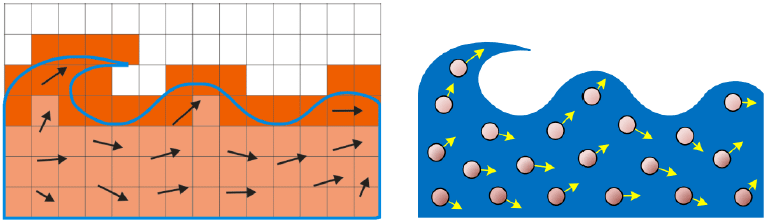
\includegraphics[scale=0.5]{images/gridBasedParticleBased}
        \caption{
            Grid based, Particle based simulation \cite{gridBasedParticleBased}
        }
        \label{fig:gridBasedParticleBased}
    \end{figure}


    \section{SPH metoda}\label{sec:sph-metoda}

    \subsection{Općenito o metodi}\label{subsec:opcenito-o-metodi}

    SPH\cite{SPHmethod} (Smoothed Particle Hydrodynamics) metoda je računska metoda koja se koristi za simulaciju fluida.
    Ova metoda je bazirana na česticama, pri čemu svaka čestica predstavlja mali volumen fluida.
    SPH metoda izračunava fizikalna svojstva fluida na temelju međučestičnih interakcija, omogućujući simulaciju fluida u složenim i nepravilnim prostorima bez potrebe za 2D poljem.

    \begin{itemize}
        \item \textbf{Osnovni princip:} U SPH metodi, prostor se ne dijeli na ćelije kao u metodama baziranim na mreži, već se koristi diskretna kolekcija čestica.
        Svaka čestica nosi informacije o fizikalnim svojstvima kao što su masa, brzina, gustoća i tlak.
        Interakcije između čestica izračunavaju se pomoću glatkih interpolacijskih funkcija, što omogućava kontinuirani prikaz fizikalnih veličina.
        \item \textbf{Prednosti:} Jedna od glavnih prednosti SPH metode je njena sposobnost da simulira fluide u složenim geometrijama i nepravilnim prostorima.
        Budući da ne koristi 2D polje, SPH metoda je fleksibilnija i može se lako prilagoditi različitim vrstama problema.
        Također, njena složenost u odnosu na broj čestica je manja nego kod metoda koje koriste 2D polje, posebno kada je gustoća čestica visoka.
        \item \textbf{Nedostaci:} Glavni nedostatak SPH metode je potreba za velikim brojem čestica kako bi se postigla visoka preciznost simulacije, što može povećati računalne zahtjeve.
        Također, postizanje stabilnosti simulacije može biti izazovno, posebno kod simulacije viskoznih i turbulentnih tokova.
    \end{itemize}

    \newpage

    \subsection{Koraci simulacije}\label{subsec:koraci-simulacije}

    \paragraphnewline{Inicijalizacija simulacije}
    Na samom početku simulacije potrebno je definirati parametre simulacije poput jačine viskoze, međučestično odbijanje i slično.

    \paragraphnewline{Traženje susjeda}

    Prvi ``pravi`` korak simulacije je traženje susjeda.
    Vrlo je važno znati susjede kako bi se na čestice mogle primjeniti sile koje ovise o udaljenosti od drugih čestica poput viskoznosti i pritiska.
    Najčešći pristup traženju susjeda su pretraga pomoću 2D polja, u kojem svaku česticu na početku simulacije spremimo u polje, te gledamo bliskost čestica koje su i bliskim poljima radi bržeg iteriranja.

    \begin{figure}[H]
        \centering
        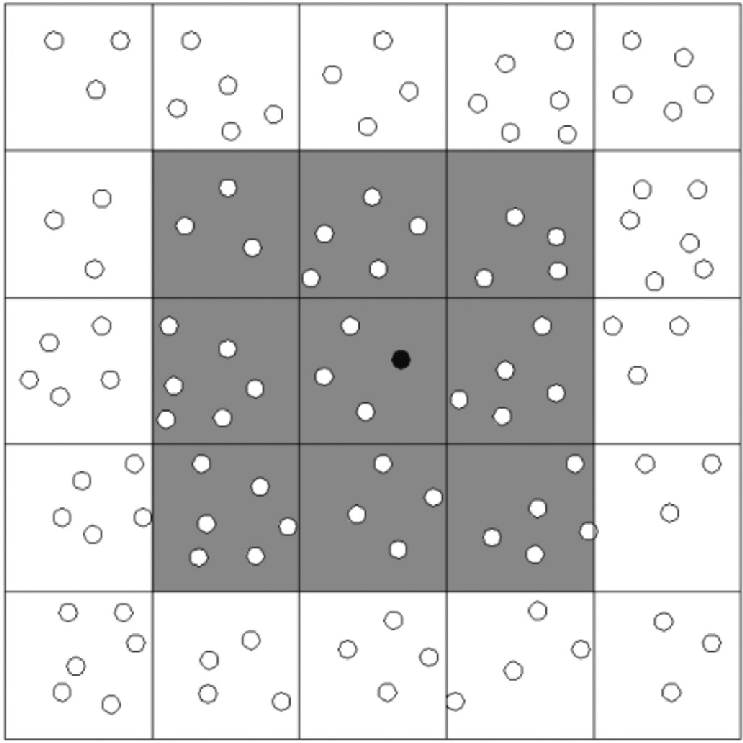
\includegraphics[scale=0.3]{images/Uniform-grid-searching-method}
        \caption{
            Uniform grid searching method \cite{uniformGridSearchingMethod}
        }
        \label{fig:uniformGridSearchingMethod}
    \end{figure}

    \newpage
    Drugi česti pristup ovome je pristup pomoću stabla, gdje se čestice spremaju u stablastu strukturu podataka i susjedi se lako traže spuštajući se niz nju.
    Susjedi se također mogu tražiti tako da se za svaku česticu ispituje udaljenost od svake druge, no složenost toga je kvadratna, te je jednostavno previše spora.

    \begin{figure}[H]
        \centering
        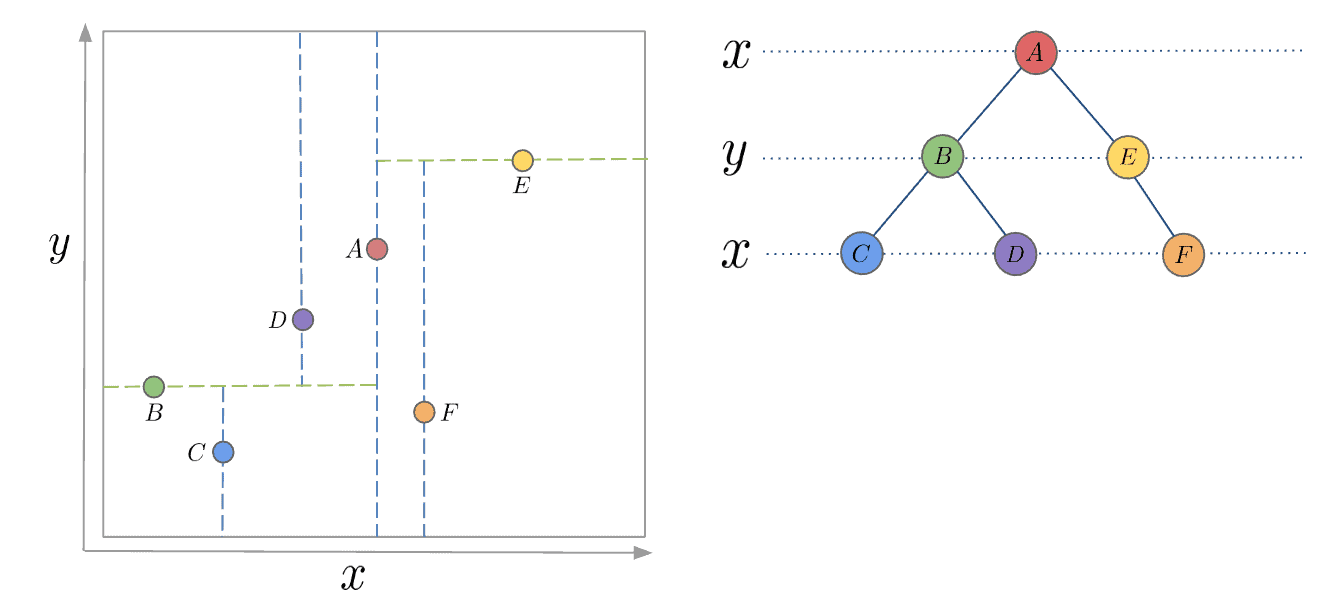
\includegraphics[scale=0.3]{images/kdtree}
        \caption{
            K-D stablo \cite{kdTree}
        }
        \label{fig:kdTree}
    \end{figure}

    \paragraphnewline{Računanje i primjena međučestičnih sila}

    Nakon pronalaska susjeda slijedi korak u kojem se računaju međučestične sile.
    Ovo je najvažniji korak jer upravo ove sile su te koje tjeraju čestice da se gibaju poput vode.
    Čestice ne smiju biti jedne u drugima, ali se svejedno moraju kretati zajedno i više čestica se mora ponašati složno.
    Najbitnije su sile sila pritiska, i sila viskoze.

    Prvo se računa gustoća, a zatim pomoću nje pritisak i onda nakon viskoza.

    Pritisak je bitan jer on tjera čestice jedne iz drugih kako nebi zapele jedna u drugu.
    \begin{figure}[H]
        \centering
        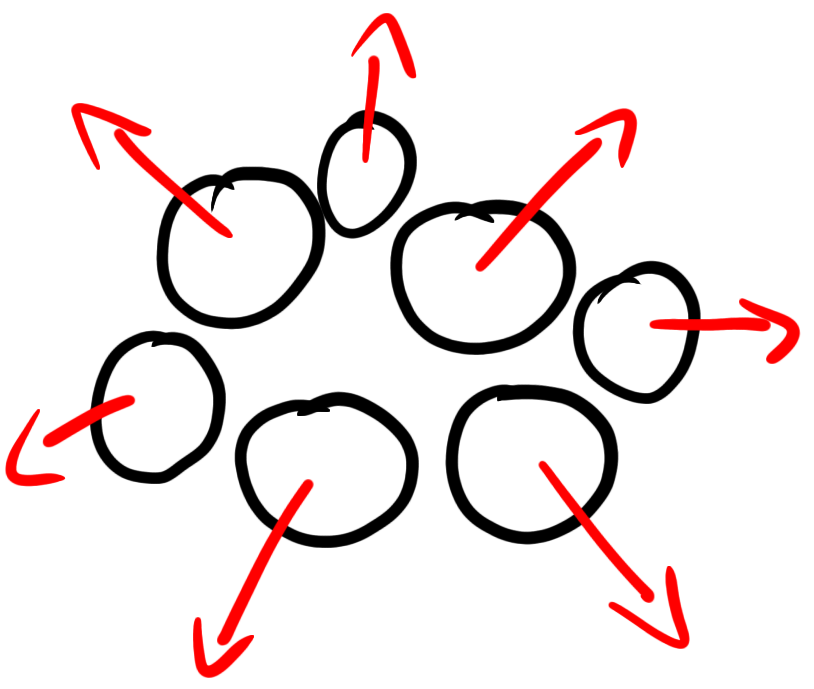
\includegraphics[scale=1]{images/pressureForce}
        \caption{
            Sile pritiska
        }
        \label{fig:pressureForce}
    \end{figure}

    \newpage
    Viskoza je suprotna pritisku, ona želi držati čestice na okupu tako da vuće čestice jedne prema drugima kako bi se micale u jednoj velikoj nakupini.
    Što je viskoza jača, fluid koji simuliramo bit će ``tvrđi`` i sve više ličiti na neku krutinu, jer će unutarnja sila biti toliko jaka da će se vanjske sile
    poput gravitacije moći zanemariti.
    \begin{figure}[H]
        \centering
        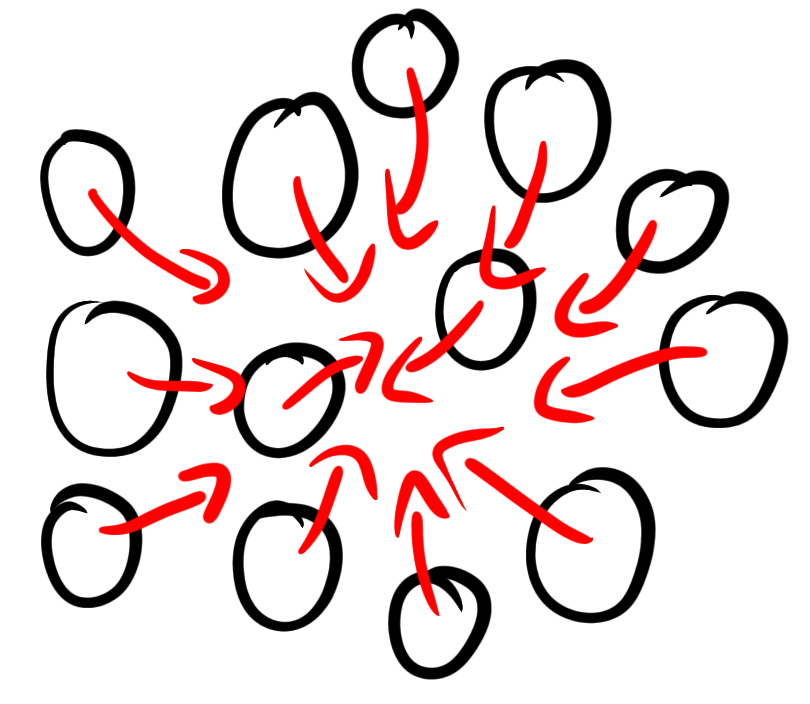
\includegraphics[scale=1]{images/viscoseForce}
        \caption{
            Sile viskoze
        }
        \label{fig:viscoseForce}
    \end{figure}


    % TODO dodat slike tih sila
    \paragraphnewline{Upravljanje rubnim uvjetima i sudarima}


    \chapter{Programska implementacija}\label{ch:programska-implementacija}


    \section{Osnove Unity okruženja}\label{sec:osnove-unity-okruzenja}


    \section{Osnove Unity fizičkog simulatora}\label{sec:osnove-unity-fizickog-simulatora}


    \section{Čestica}\label{sec:cestica}


    \section{Gustoća}\label{sec:gustoca}


    \section{Pritisak}\label{sec:pritisak}


    \section{Viskoza}\label{sec:viskoza}


    \section{Rezultantna sila}\label{sec:rezultantna-sila}


    \bibliography{literatura}
    \begin{sazetak}
        sažetak na hrvatskom
    \end{sazetak}
    \begin{kljucnerijeci}
        ključne riječi na hrvatskom
    \end{kljucnerijeci}
    \begin{abstract}
        abstract in English
    \end{abstract}
    \begin{keywords}
        keywords in English
    \end{keywords}
\end{document}